% !Mode::"TeX:UTF-8"
\documentclass[a4paper]{article}
\usepackage{amssymb}
\usepackage{geometry}
\usepackage{graphicx}
\usepackage{fancyhdr}
\usepackage{setspace}
\usepackage{pdfpages}
\usepackage{listings}
\usepackage{amsthm}
\usepackage{url}
\usepackage{hyperref}
\usepackage{subcaption}

\graphicspath{{./figure/}}

\geometry{left=2.5cm,right=2.5cm,top=2.5cm,bottom=2.5cm}

\author{Chi Zhang\\\\USC ID: 6099-4134-05\\\\Department of Computer Science\\\\University of Southern California}
\title{CSCI 699 Spring 2019\\Machine Learning for Knowledge Extraction \& Reasoning\\Homework 1\thanks{Instructor: Xiang Ren}}

\begin{document}

  \maketitle                     %generate the title
  \begin{spacing}{1.5}
 
  \section{Code Repository}
  \url{https://github.com/vermouth1992/CSCI699ml4know/tree/master/hw1}
 
  \section{Conditional Random Field}
  We train conditional random field model using external library sklearn-crfsuite \cite{sklearn_crfsuite} by following the tutorial \url{https://eli5.readthedocs.io/en/latest/tutorials/sklearn_crfsuite.html}. The main goal in this part is to explore the effect of various features and use them for the RNN-based model.
  \subsection{Feature Selection}
  We follow \cite{ner_features} and the tutorial and select the following set of features:
  \begin{enumerate}
    \item The word itself, last three characters and last two characters.
    \item Whether the word is uppercase.
    \item Whether the word is title. The word is title if the string is a titlecased string and there is at least one character, for example uppercase characters may only follow uncased characters and lowercase characters only cased ones. We use Python builtin function istitle().
    \item Whether the word is digit.
    \item Whether the word is float.
    \item Whether the word contains hyphen.
    \item The Part-of-Speech tag of the word.
    \item The context of the word. We follow \cite{ner_features} by using a window size of 3 that is shown to work best.
  \end{enumerate}

  We use 25\% of the training sentences as validation sentences. We measure the F1 score on validation sentences and testa sentences by adding the feature one by one. All the models are trained using LBFGS optimization with 100 iterations.

  \subsection{Result}
  \begin{table}
    \centering
    \caption{Performance of various features using CRF}
    \begin{tabular}{|c|c|c|}
      \hline
      Features Set & Validation F1 & Testa F1 \\\hline
      1   & 68.05 & 63.26 \\\hline
      1 - 2 & 68.02 &  63.01\\\hline
      1 - 3 & 73.30 & 68.05 \\\hline
      1 - 4 & 73.33 &  68.21 \\\hline
      1 - 5 & 73.44 &  67.87 \\\hline
      1 - 6 & 73.37 & 67.60 \\\hline
      1 - 7 & 75.47 & 69.52 \\\hline
      1 - 8 & 79.64 & 76.12  \\\hline
    \end{tabular}
  \label{table:crf_performance}
  \end{table}
  
  We show the validation F1-score and testa data F1-score for models using various features in Table~\ref{table:crf_performance}. We summarize the most important features as follows:
  \begin{itemize}
    \item By adding "istitle" feature, the performance boosts by 5\%.
    \item By adding "POStag" feature, the performance boosts by 2\%.
    \item By adding "context" feature, the performance boosts around 6\%.
  \end{itemize}
   To analyze which label benefits from those features, we show label-specific performance of important features in Figure~\ref{fig:label_specific_performance}.
   B-FAC and B-LAW benefits a lot from istitle feature. This is because most B-FAC and B-LAW starts with capitalized characters such as Article-II and Education Improvement. The boost of Postag comes from B-Person, B-ORG, B-NORP and B-LOC. This is because most of these labeled word is NNP. The context feature is crucial important for I-tag because I-tag always comes after B-tag.
  
  \begin{figure*}[t!]
    \centering
    \begin{subfigure}[t]{0.5\textwidth}
      \centering
      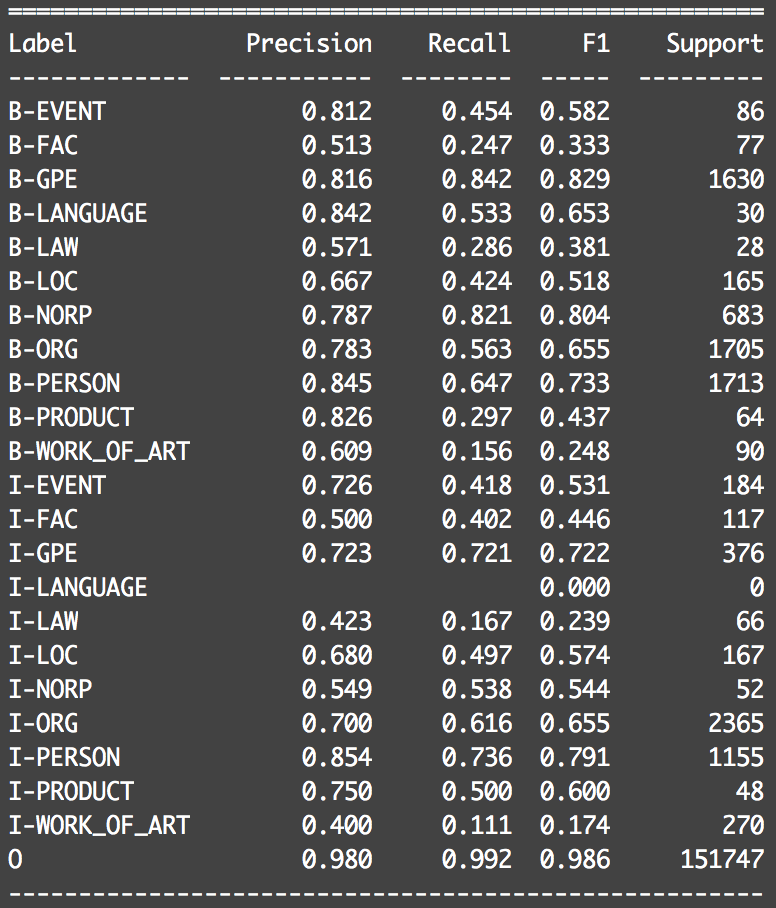
\includegraphics[width=\linewidth]{log_no_title}
      \caption{Feature set 1 - 2 (No istitle)}
    \end{subfigure}%
    ~ 
    \begin{subfigure}[t]{0.5\textwidth}
      \centering
      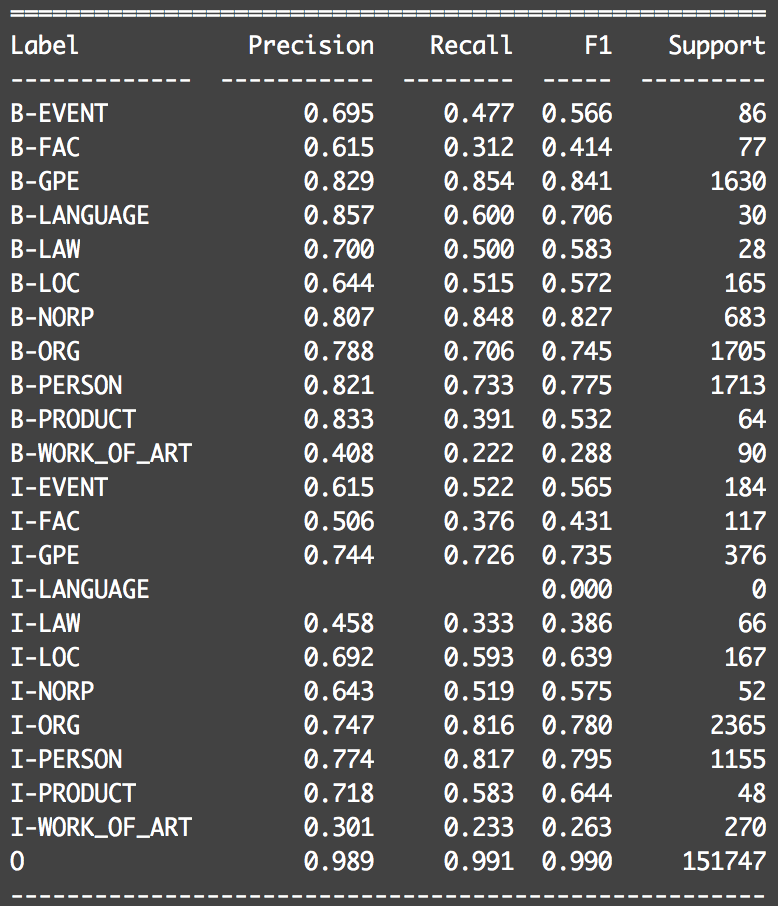
\includegraphics[width=\linewidth]{log_no_postag}
      \caption{Feature set 1 - 6 (No POStag)}
    \end{subfigure}
    ~ 
    \begin{subfigure}[t]{0.48\textwidth}
      \centering
      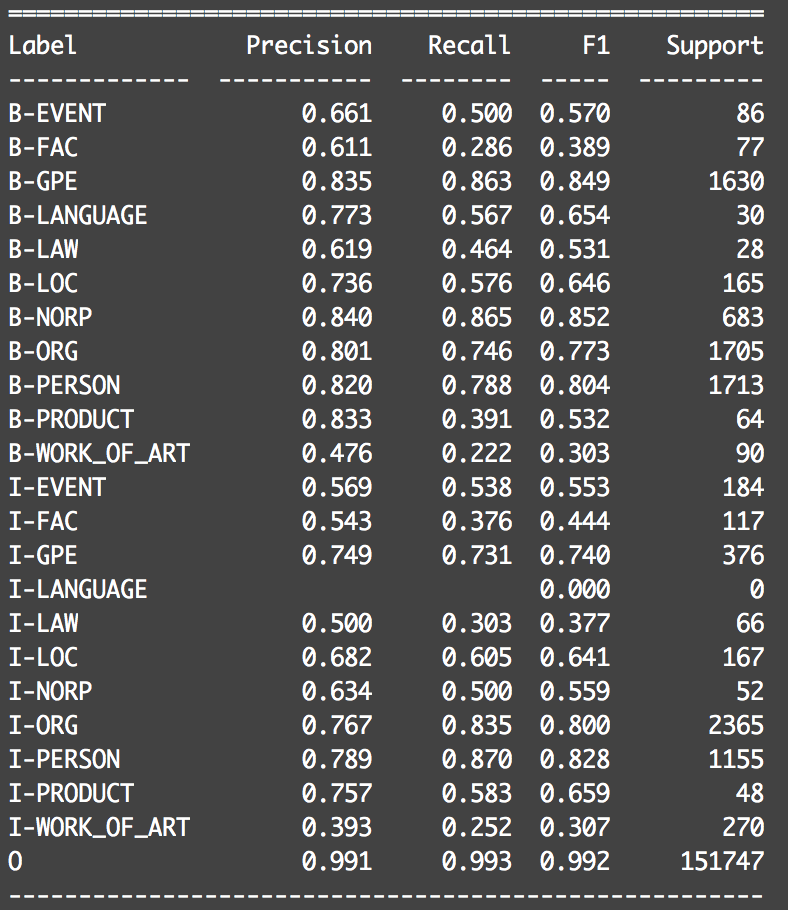
\includegraphics[width=\linewidth]{log_no_context}
      \caption{Feature set 1 - 7 (No context)}
    \end{subfigure}
    ~ 
    \begin{subfigure}[t]{0.48\textwidth}
      \centering
      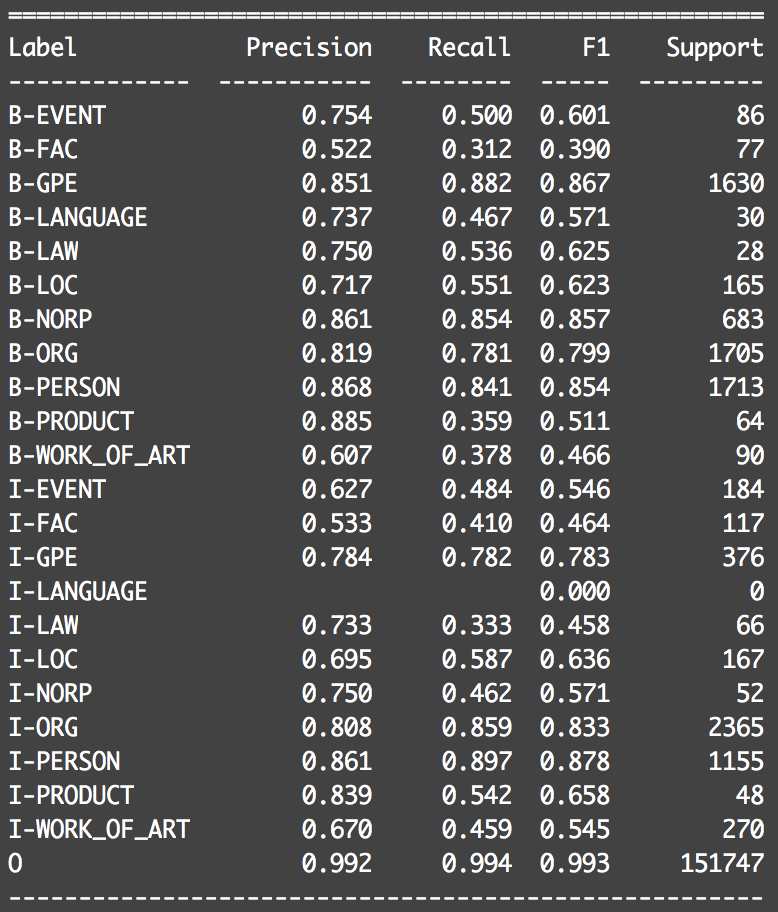
\includegraphics[width=\linewidth]{log_all_feature}
      \caption{Feature set 1 - 8 (All)}
    \end{subfigure}
    \caption{Label-specific performance of various features}
    \label{fig:label_specific_performance}
  \end{figure*}
  
  
  \section{RNN-based Model}
  \subsection{Overview}
  We implement RNN-based model using Pytorch version 1.0.0. We use GloVe \cite{glove} to initialize the embedding. After the embedding layer, we try BiLSTM vs. CNN layer followed by a fully-connected layer with softmax activation.
  
  \subsection{Architecture Comparison}
  \subsubsection{CNN vs BiLSTM}
  The number of layer is 1 for both architecture. The filter size of CNN is 3 and hidden size for both architecture is 64. The learning rate is set to 1e-3. The F1 score of CNN on testa data is 66.39\% and the F1 score of BiLSTM on testa data is 70.77\%. The approximate 4\% performance boost indicates that name entity tags generally have long-term dependency instead of depending purely on local context words.
  
  \subsection{Additional Features}
  The word embedding can be viewed as features for the word itself. By using CNN or BiLSTM, we include features for context words. Like conditional random fielf, we add additional features including istitle, isdigit and isupper and part-of-speech tag to BiLSTM model and the F1 score on testa is 71.12\%.
  
  \subsection{Number of Layers}
  We try 2 layer and 3 layer BiLSTM with 50\% dropout. The F1 performance on testa dataset is 73.65\% and 72.41\%. The model becomes more and more overfitting by adding more layers.
  
  \subsection{Embedding Comparison}
  We try to use contextual embedding BERT \cite{bert} without case to finetune a transformer model based on tutorial \url{https://www.depends-on-the-definition.com/named-entity-recognition-with-bert/}. However, the final performance on testa data is only around 67\% and it's hard to analyze what's going wrong.
  
  \subsection{Additional thoughts}
  GloVe and BERT is uncased embedding, which ignore the difference between Education Improvement and education improvement. However, as shown in Part 1, the character-level feature plays an important role in name entity recognition. Thus, we believe there would be huge performance boost by adding char-level features such as using CNN as extractor. Due to limited time, we leave this to future work.
  
  \end{spacing}  
  \bibliographystyle{abbrv}
  \bibliography{./bib/chizhang.bib}

\end{document}
